\documentclass[a4paper,12pt]{article}

\usepackage[T2A]{fontenc}			
\usepackage[utf8]{inputenc}			
\usepackage[english,russian]{babel}	

\usepackage[
bookmarks=true, colorlinks=true, unicode=true,
urlcolor=black,linkcolor=black, anchorcolor=black,
citecolor=black, menucolor=black, filecolor=black,
]{hyperref}

\usepackage{color}
\usepackage{caption}
\DeclareCaptionFont{white}{\color{black}}
\DeclareCaptionFormat{listing}{\colorbox{white}{\parbox{\textwidth}{#1#2#3}}}
\captionsetup[lstlisting]{format=listing,labelfont=white,textfont=white}

\usepackage{amsmath,amsfonts,amssymb,amsthm,mathtools} 
\usepackage{wasysym}

\usepackage{graphicx}
%\usepackage[cache=false]{minted}
\usepackage{cmap}
\usepackage{indentfirst}

\usepackage{listings} 
\usepackage{fancyvrb}

\usepackage{geometry}
\geometry{left=2cm}
\geometry{right=1.5cm}
\geometry{top=1cm}
\geometry{bottom=2cm}

\setlength{\parindent}{5ex}
\setlength{\parskip}{0.5em}

\usepackage{pgfplots}
\usetikzlibrary{datavisualization}
\usetikzlibrary{datavisualization.formats.functions}

\begin{document}
	\lstset{ %
		language=C,                 % выбор языка для подсветки (здесь это С)
		basicstyle=\small\sffamily, % размер и начертание шрифта для подсветки кода
		numbers=left,               % где поставить нумерацию строк (слева\справа)
		numberstyle=\tiny,           % размер шрифта для номеров строк
		stepnumber=1,                   % размер шага между двумя номерами строк
		numbersep=5pt,                % как далеко отстоят номера строк от подсвечиваемого кода
		backgroundcolor=\color{white}, % цвет фона подсветки - используем \usepackage{color}
		showspaces=false,            % показывать или нет пробелы специальными отступами
		showstringspaces=false,      % показывать или нет пробелы в строках
		showtabs=false,             % показывать или нет табуляцию в строках
		frame=single,              % рисовать рамку вокруг кода
		tabsize=2,                 % размер табуляции по умолчанию равен 2 пробелам
		captionpos=t,              % позиция заголовка вверху [t] или внизу [b] 
		breaklines=true,           % автоматически переносить строки (да\нет)
		breakatwhitespace=false, % переносить строки только если есть пробел
		escapeinside={\%*}{*)}   % если нужно добавить комментарии в коде
	}
	
	% Титульный лист
	\begin{figure}[h!]
		\begin{center}
			{
\includegraphics[scale = 0.4]{titul.jpg}}
			\label{titul}
		\end{center}
	\end{figure}
	
	\vspace*{15mm} 
	
	\huge
	\begin{center}
		Дисциплина: <<Операционные системы>>
	\end{center}
	
	\begin{center}
		Лабораторная работа №5
	\end{center}

	
	\huge
	\begin{center}
		Тема работы:\\
		<<Буферизованный и небуферизованный
		ввод-вывод>>
	\end{center}
	\vspace*{30mm} 
	
	\large
	\begin{flushright}
		Студент: Левушкин И. К. \\
		Группа: ИУ7-62Б \\
		Преподаватель: Рязанова Н. Ю. \\
	\end{flushright}
	
	\vspace*{30mm}
	\begin{center}
		Москва, 2020 г.  
	\end{center}
	\thispagestyle{empty}
	
	
	\newpage
	
	\section*{Задание}
	
	В лабораторной работе анализируется результат выполнения трех программ. Программы демонстрируют открытие одного и того же файла
	несколько раз. Реализация открытия файла в одной программе несколько раз выбрана для простоты. Такая ситуация возможна в системе, когда
	один и тот же файл несколько раз открывают разные процессы. Но для получения ситуаций аналогичных тем, которые демонстрируют приведенные
	программы надо было бы синхронизировать работу процессов. При выполнении асинхронных процессов такая ситуация вероятна и ее надо учитывать, чтобы избежать потери данных или получения неверного результата
	при выводе в файл.
	
	\newpage
	
	\section*{1 программа}
	
	\begin{figure}[h!]
		\begin{center}
			{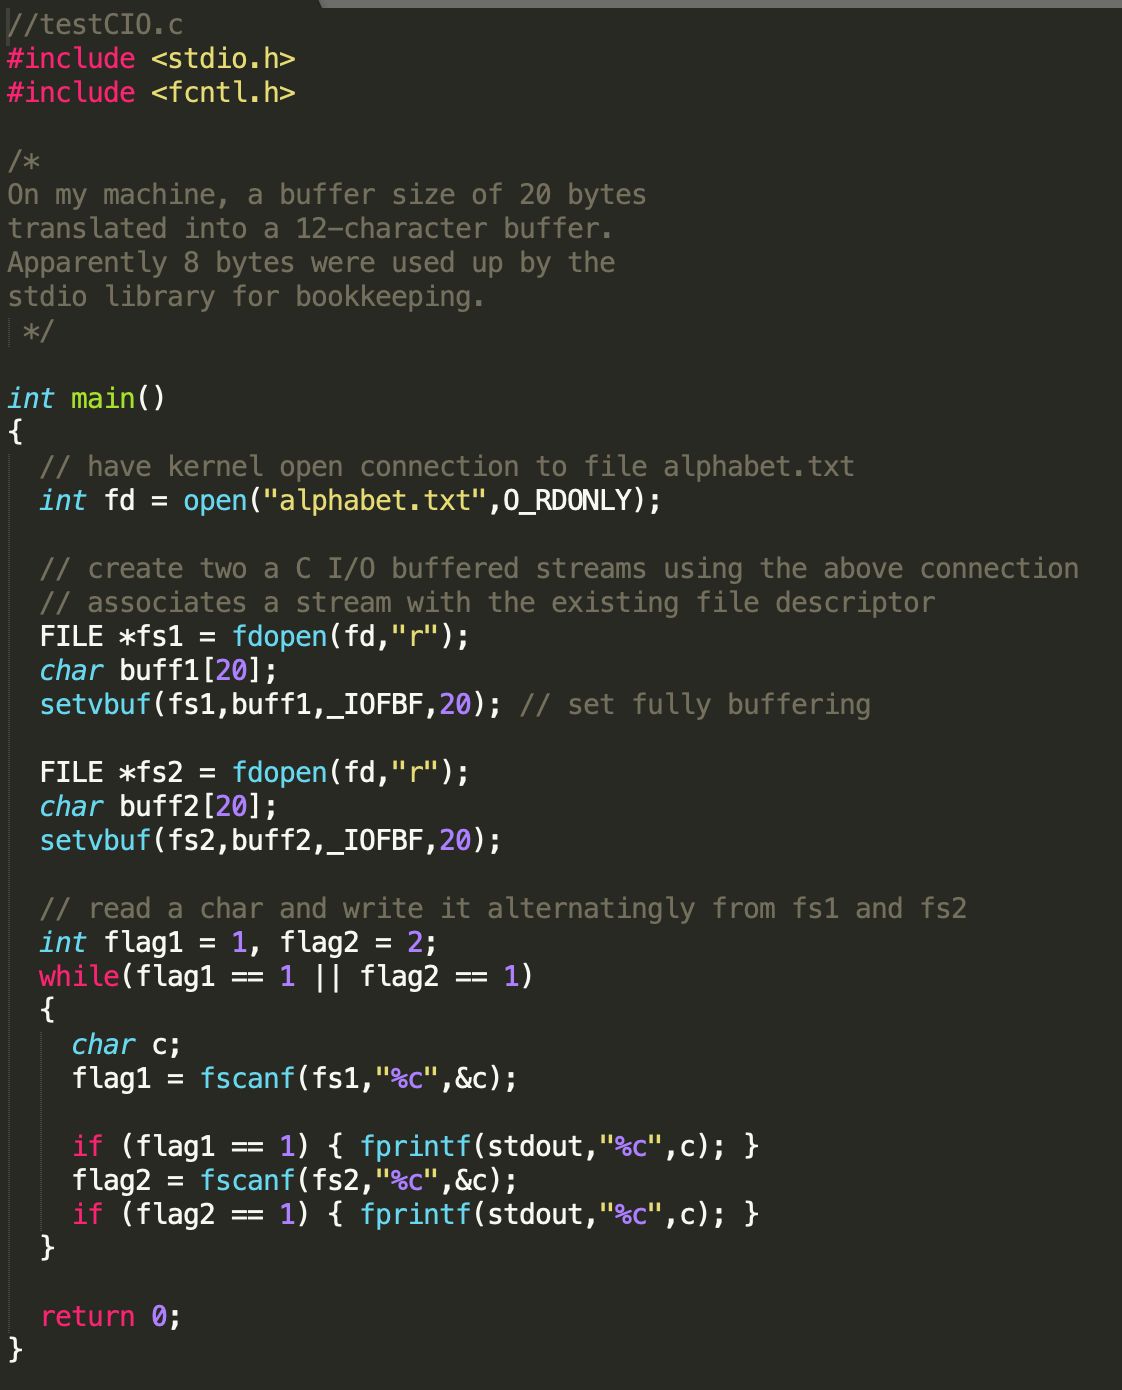
\includegraphics[scale = 0.7]{testCIO.png}}
			\label{ris:testCIO}
		\end{center}
	\end{figure}
	
	Результат работы:
	
	\begin{lstlisting}[label = lst1, caption =  Результат testCIO.out]
	Aubvcwdxeyfzghijklmnopqrst
	\end{lstlisting}
	
	\newpage
	
	\begin{figure}[h!]
		\begin{center}
			{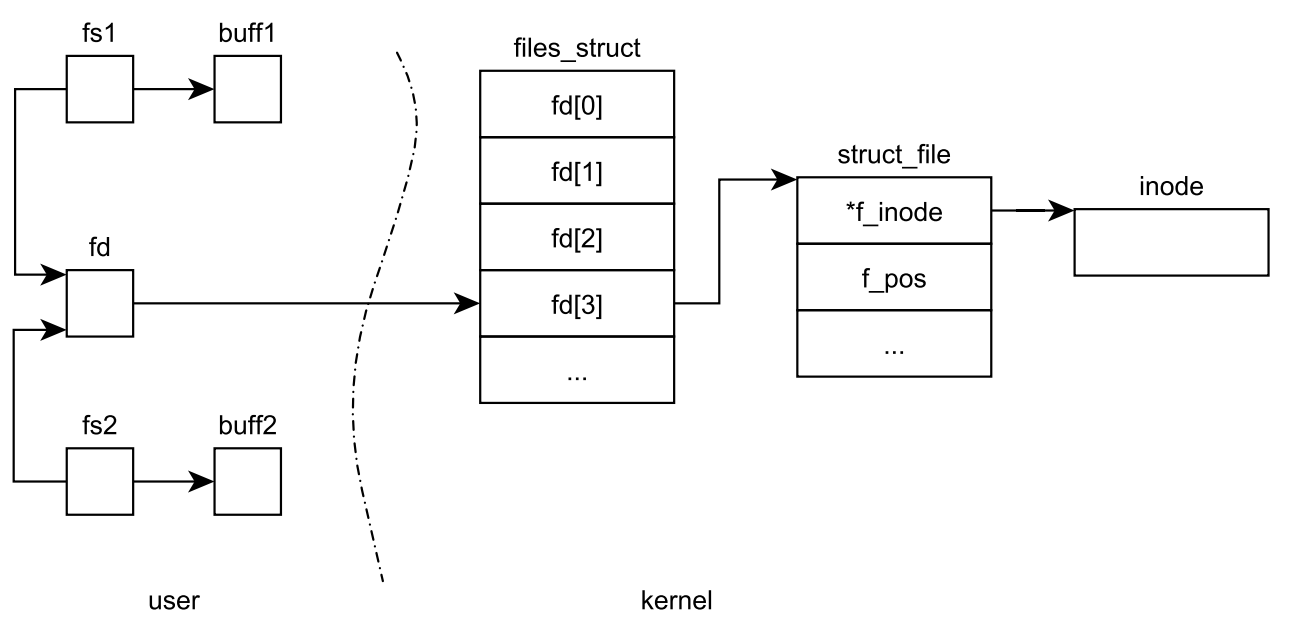
\includegraphics[scale = 0.7]{page1.png}}
			\label{ris:page1}
		\end{center}
		\caption{Связь дескрипторов в программе 1}
	\end{figure}
	
	С помощью системного вызова \textit{open()} создается дискриптор файла, при
	этом файл открывается только на чтение (флаг \textit{O\_RDONLY}), указатель устанавливается на начало файла. Если системный вызов завершается успешно, возвращенный файловый дескриптор является наименьшим, который еще не открыт
	процессом. В результате этого вызова появляется новый открытый файл, не
	разделяемый никакими процессами, и запись в системной таблице открытых
	файлов.
	
	Затем с помощью функции \textit{fdopen()} создаются два потока данных \textit{fs1}
	и \textit{fs2}, которые связываются с файлом, описанным дескриптором \textit{fd}. Функция
	\textit{setvbuf()} изменяет тип буферизации на блочную (полную) размером в 20 байт.
	
	В цикле осуществеляется чтение из потоков (функция \textit{fscanf()}) и вывод
	в \textit{stdout} (функция \textit{fprintf()}). Флаги \textit{flag1} и \textit{flag2} изменят свое значение
	3
	с 1 на -1 тогда, когда число прочитанных символов станет равно нулю. Вследствие буферизации в \textit{buff1} фактически помещается строка \textit{Abcdefghijklmnopqrst}
	– первые 20 символов, а в \textit{buff2} – \textit{uvwxyz} – оставшаяся часть (при первом чтении
	указатель в файле сместился на 20 символов). Отсюда получаем соответствующий результат (листинг \ref{lst1}).
	
	\newpage
	
	\section*{2 программа}
	
	\begin{figure}[h!]
		\begin{center}
			{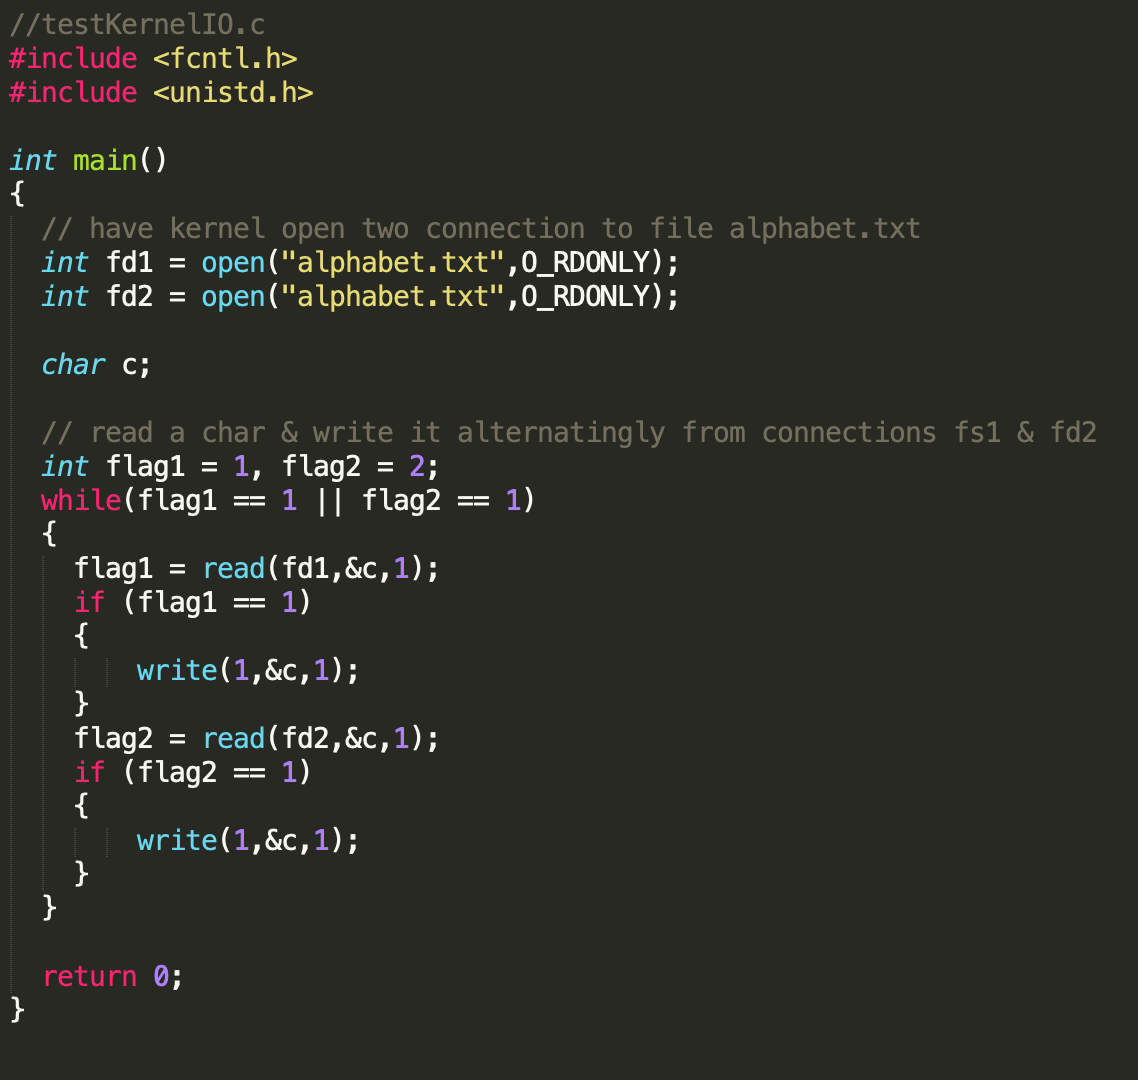
\includegraphics[scale = 0.7]{testKernelIO.png}}
			\label{ris:testKernelIO}
		\end{center}
	\end{figure}
	
	Результат работы программы:
	
	\begin{lstlisting}[label = lst2, caption = Результат testKernelIO.out]
	AAbbccddeeffgghhiijjkkllmmnnooppqqrrssttuuvvwwxxyyzz
	\end{lstlisting}
	
	Здесь создаются два файловых дескриптора и две разные записи в системной таблице открытых файлов. Файловые дескрипторы независимы друг от друга, поэтому положения указателей в файле также независимы.
	
	В цикле с помощью системных вызовов \textit{read()} и \textit{write()} посимвольно происходит чтение из файла и запись в стандартный поток вывода соответственно.
	Поэтому получаем строку с дублирующимися буквами (листинг \ref{lst2}).
	
	\newpage
		
	\begin{figure}[h!]
		\begin{center}
			{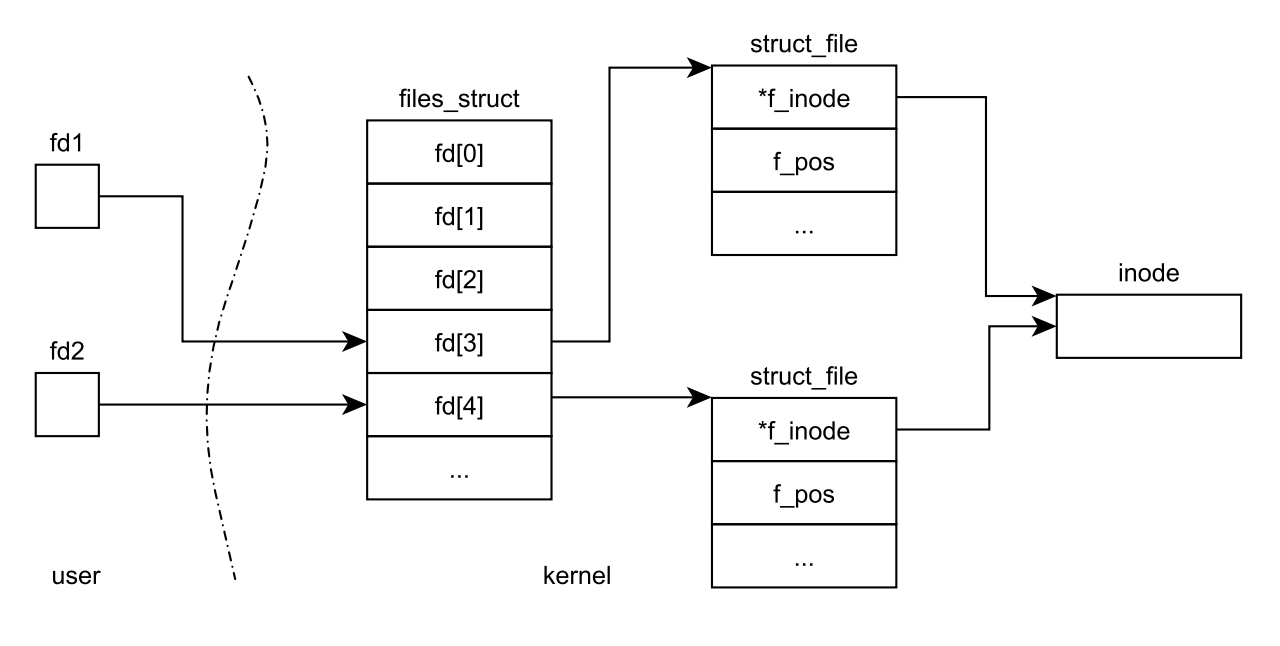
\includegraphics[scale = 0.7]{page2.png}}
			\label{ris:page2}
		\end{center}
		\caption{Связь дескрипторов в программе 2}
	\end{figure}
		
	\newpage
		
	\section*{3 программа}
	
	\begin{figure}[h!]
		\begin{center}
			{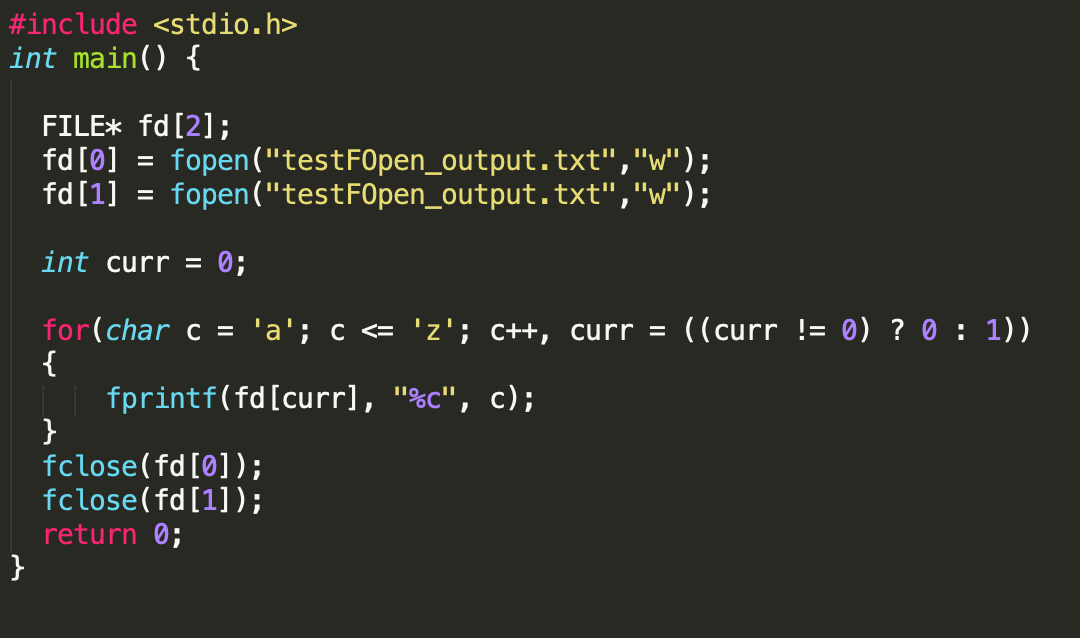
\includegraphics[scale = 0.7]{testFopen.png}}
			\label{ris:testFopen}
		\end{center}
	\end{figure}
	
	Результат работы программы:
	
	\begin{lstlisting}[label = lst3, caption = Результат testFopen.out]
	bdfhjlnprtvxz
	\end{lstlisting}
	
	\begin{figure}[h!]
		\begin{center}
			{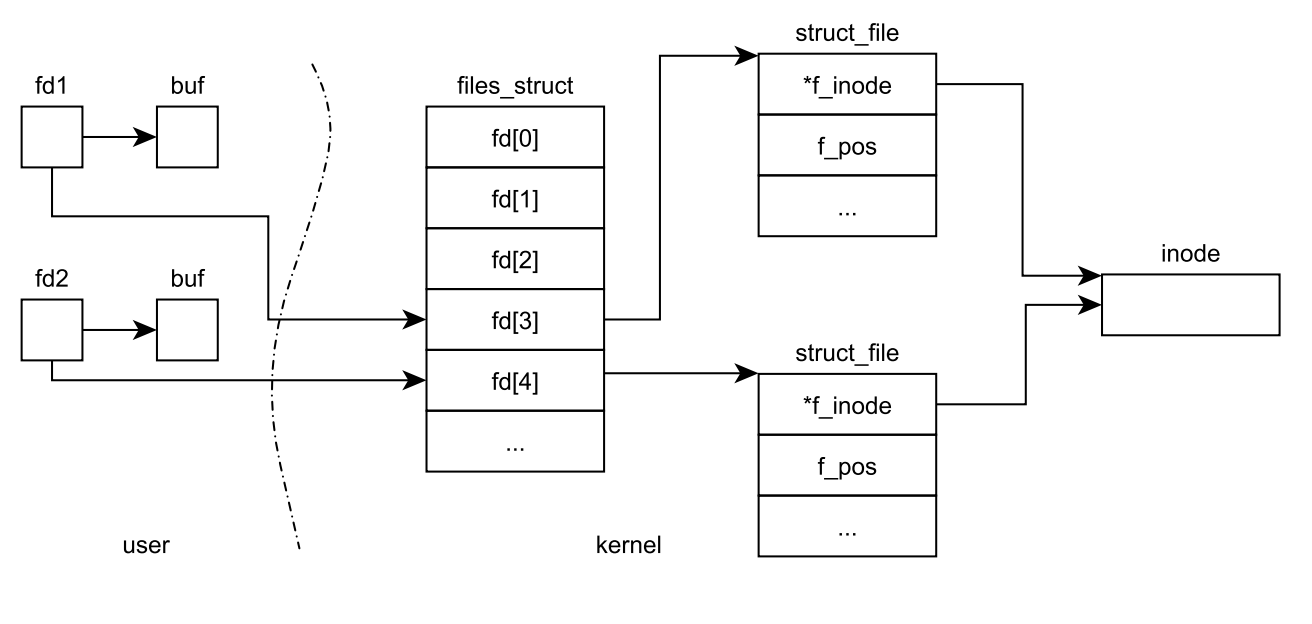
\includegraphics[scale = 0.7]{page3.png}}
			\label{ris:page3}
		\end{center}
		\caption{Связь дескрипторов в программе 3}
	\end{figure}
	
	С помощью функций \textit{fopen()} открываются два потока на запись с начала
	файла. Они имеют два разных файловых дескриптора, а значит и независимые
	позиции в файле.
	
	В цикле с помощью \textit{fprintf()} в потоки поочередно записываются буквы
	от \textit{a} до \textit{z} (нечетные – в первый поток, четные – во второй). Как было отмечено
	ранее, функция \textit{fprintf()} обеспечивает буферизацию. Запись в файл происходит либо при полном заполнении буфера, либо при вызове функций \textit{fclose()}
	или   \textit{fflush()}.
	
	Таким образом, когда в программе происходит вызов функции \textit{fclose(fd1)}, в файл записываются данные первого потока, однако далее после вызова функции \textit{fclose(fd2)} содержимое файла удаляется (ранее был установлен режим
	записи) и записывается информация из буфера второго потока.
	
	\section*{Структура FILE}
	
	\begin{lstlisting}[label = lst4, caption = Структура FILE]
	// "bits/types/FILE.h"
	
	#ifndef __FILE_defined
	#define __FILE_defined 1
	
	struct _IO_FILE;
	
	/*
		The opaque type of streams. This is the definition used elsewhere.
	*/
	
	typedef struct _IO_FILE FILE;
	
	#endif
	
	...
	
	// "bits/libio.h"
	
	struct _IO_FILE
	{
		int _flags;                /* High-order word is _IO_MAGIC; rest is flags. */
		/* The following pointers correspond to the C++ streambuf protocol. */
		char *_IO_read_ptr;        /* Current read pointer */
		char *_IO_read_end;        /* End of get area. */
		char *_IO_read_base;        /* Start of putback+get area. */
		char *_IO_write_base;        /* Start of put area. */
		char *_IO_write_ptr;        /* Current put pointer. */
		char *_IO_write_end;        /* End of put area. */
		char *_IO_buf_base;        /* Start of reserve area. */
		char *_IO_buf_end;        /* End of reserve area. */
		/* The following fields are used to support backing up and undo. */
		char *_IO_save_base; /* Pointer to start of non-current get area. */
		char *_IO_backup_base;  /* Pointer to first valid character of backup area */
		char *_IO_save_end; /* Pointer to end of non-current get area. */
		struct _IO_marker *_markers;
		struct _IO_FILE *_chain;
		int _fileno;
		int _flags2;
		__off_t _old_offset; /* This used to be _offset but it's too small.  */
		/* 1+column number of pbase(); 0 is unknown. */
		unsigned short _cur_column;
		signed char _vtable_offset;
		char _shortbuf[1];
		_IO_lock_t *_lock;
		#ifdef _IO_USE_OLD_IO_FILE
	};
	\end{lstlisting}
	
	\section*{Вывод}
	
	Из проделанной работы можно сделать следующие выводы:
	
	\begin{enumerate}
		\item При буферизованном вводе (выводе) необходимо учитывать, что запись
		(чтение) происходит именно из буфера. Поэтому неправильные действия
		могут привести к неверной обработке данных или даже к потере информации, что и было продемонстрировано в 1 и 3 программах. В 3 программе запись в файл осуществлялась с помощью функции fclose(), в результате чего при повторном ее вызове для второго потока содержимое файла, записанное первым потоком, удалялось и записывалась информация из буфера второго потока. В следствие чего терялась ранее записанная информация.
		\item При небуферизованном вводе (выводе) стоит учесть, что при одновременном открытии одного и того же файла создается столько дескрипторов и записей в таблице открытых файлов, сколько раз был открыт файл. Каждый дескриптор \textit{struct\_file} имеет поле \textit{f\_pos}, указывающее на позицию чтения (записи) в файле, независящую от других дескрипторов. Это и позволяет процессам обрабатывать файл независимо друг от друга. Таким образом, чтение из файла будет происходить нормально, но при попытке одновременно писать в один файл при небуферизованном вводе (выводе) будет получаться неправильный результат, смешанный из того, что хотели напечатать. Это и было продемонстрировано в 2 программе: 
		
		хотели напечатать: \textit{AbcdefghijklmnopqrstuvwxyzAbcdefghijklmnopqrstuvwxyz},
		
		получили: \textit{AAbbccddeeffgghhiijjkkllmmnnooppqqrrssttuuvvwwxxyyzz}.
		\item Поэтому необходимо четко понимать разницу между функциями из стандартной библиотеки C, обеспечивающих буферизованный ввод-вывод и системными вызовами с небуферизованным вводом-выводом.
	\end{enumerate}

	
\end{document}